\newif\ifdraft

\draftfalse

\ifdraft
	\documentclass[10pt, a4paper]{article}
	\addtolength{\oddsidemargin}{-.875in}
	\addtolength{\evensidemargin}{-.875in}
	\addtolength{\textwidth}{1.75in}
	\addtolength{\topmargin}{-.875in}
	\addtolength{\textheight}{1.75in}
\else
	\newcommand{\svcourse}{$$TRIPOS$$: $$COURSE$$}
\newcommand{\svnumber}{$$SVNUM$$}
\newcommand{\svvenue}{$$VENUE$$}
\newcommand{\svdate}{$$SVDATE$$}
\newcommand{\svtime}{$$SVTIME$$}
\newcommand{\svuploadkey}{$$SVUPLOADKEY$$}

\newcommand{\svrname}{$$SVR_NAME$$}
\newcommand{\jkfside}{$$SVR_PAPER_SIDED$$}
\newcommand{\jkfhanded}{$$SVR_PAPER_HANDED$$}

\newcommand{\studentname}{$$STU_NAME$$}
\newcommand{\studentemail}{$$STU_EMAIL$$}


	\documentclass[10pt,\jkfside,a4paper]{article}
	% DO NOT add \usepackage commands here.  Place any custom commands
% into your SV work files.  Anything in the template directory is
% likely to be overwritten!

\usepackage{fancyhdr}

\usepackage{lastpage}       % ``n of m'' page numbering
\usepackage{lscape}         % Makes landscape easier

\usepackage{verbatim}       % Verbatim blocks
\usepackage{listings}       % Source code listings
\usepackage{epsfig}         % Embed encapsulated postscript
\usepackage{array}          % Array environment
\usepackage{qrcode}         % QR codes
\usepackage{enumitem}       % Required by Tom Johnson's exam question header

\usepackage{hhline}         % Horizontal lines in tables
\usepackage{siunitx}        % Correct spacing of units
\usepackage{amsmath}        % American Mathematical Society
\usepackage{amssymb}        % Maths symbols
\usepackage{amsthm}         % Theorems

\usepackage{ifthen}         % Conditional processing in tex

\usepackage[top=3cm,
            bottom=3cm,
            inner=2cm,
            outer=5cm]{geometry}

% PDF metadata + URL formatting
\usepackage[
            pdfauthor={\studentname},
            pdftitle={\svcourse, SV \svnumber},
            pdfsubject={},
            pdfkeywords={9d2547b00aba40b58fa0378774f72ee6},
            pdfproducer={},
            pdfcreator={},
            hidelinks]{hyperref}



\renewcommand{\headrulewidth}{0.4pt}
\renewcommand{\footrulewidth}{0.4pt}
\fancyheadoffset[LO,LE,RO,RE]{0pt}
\fancyfootoffset[LO,LE,RO,RE]{0pt}
\pagestyle{fancy}
\fancyhead{}
\fancyhead[LO,RE]{{\bfseries \studentname}\\\studentemail}
\fancyhead[RO,LE]{{\bfseries \svcourse, SV~\svnumber}\\\svdate\ \svtime, \svvenue}
\fancyfoot{}
\fancyfoot[LO,RE]{For: \svrname}
\fancyfoot[RO,LE]{\today\hspace{1cm}\thepage\ / \pageref{LastPage}}
\fancyfoot[C]{\qrcode[height=0.8cm]{\svuploadkey}}
\setlength{\headheight}{22.55pt}


\ifthenelse{\equal{\jkfside}{oneside}}{

 \ifthenelse{\equal{\jkfhanded}{left}}{
  % 1. Left-handed marker, one-sided printing or e-marking, use oneside and...
  \evensidemargin=\oddsidemargin
  \oddsidemargin=73pt
  \setlength{\marginparwidth}{111pt}
  \setlength{\marginparsep}{-\marginparsep}
  \addtolength{\marginparsep}{-\textwidth}
  \addtolength{\marginparsep}{-\marginparwidth}
 }{
  % 2. Right-handed marker, one-sided printing or e-marking, use oneside.
  \setlength{\marginparwidth}{111pt}
 }

}{
 % 3. Alternating margins, two-sided printing, use twoside.
}


\setlength{\parindent}{0em}
\addtolength{\parskip}{1ex}

% Exam question headings, labels and sensible layout (courtesy of Tom Johnson)
\setlist{parsep=\parskip, listparindent=\parindent}
\newcommand{\examhead}[3]{\section{#1 Paper #2 Question #3}}
\newenvironment{examquestion}[3]{
\examhead{#1}{#2}{#3}\setlist[enumerate, 1]{label=(\alph*)}\setlist[enumerate, 2]{label=(\roman*)}
\marginpar{\href{https://www.cl.cam.ac.uk/teaching/exams/pastpapers/y#1p#2q#3.pdf}{\qrcode{https://www.cl.cam.ac.uk/teaching/exams/pastpapers/y#1p#2q#3.pdf}}}
\marginpar{\footnotesize \href{https://www.cl.cam.ac.uk/teaching/exams/pastpapers/y#1p#2q#3.pdf}{https://www.cl.cam.ac.uk/\\teaching/exams/pastpapers/\\y#1p#2q#3.pdf}}
}{}


\fi

\newcommand\ddfrac[2]{\frac{\displaystyle #1}{\displaystyle #2}}
\newcommand\tx\textrm

\begin{document}

\begin{enumerate}

\item 
\begin{enumerate}

\item 
Lec. 3 Ex. 1,2
\begin{enumerate}
	\item Define $e \in \text{Halt}_{X \times Y}$ if $e$ halts and 
	$(fst(e) \in \text{Halt}_X ) \wedge (snd(e) \in \text{Halt}_Y )$
	
	
	\item Define $e \in \text{Halt}_{X+Y}$ if $e$ halts and  
	$((\forall e''' \in \text{Halt}_X . [e'''/x]e' \in \text{Halt}_Z ) \wedge (\forall e''' \in \text{Halt}_Y . [e'''/y]e'' \in \text{Halt}_Z )) \rightarrow 
	\verb|case(e, Lx -> e', Ry -> e'')| \in \text{Halt}_Z $ \\
	
\end{enumerate}


\item 
Lec 5. Ex
\begin{enumerate}
	\item Regularity Lemma \\
	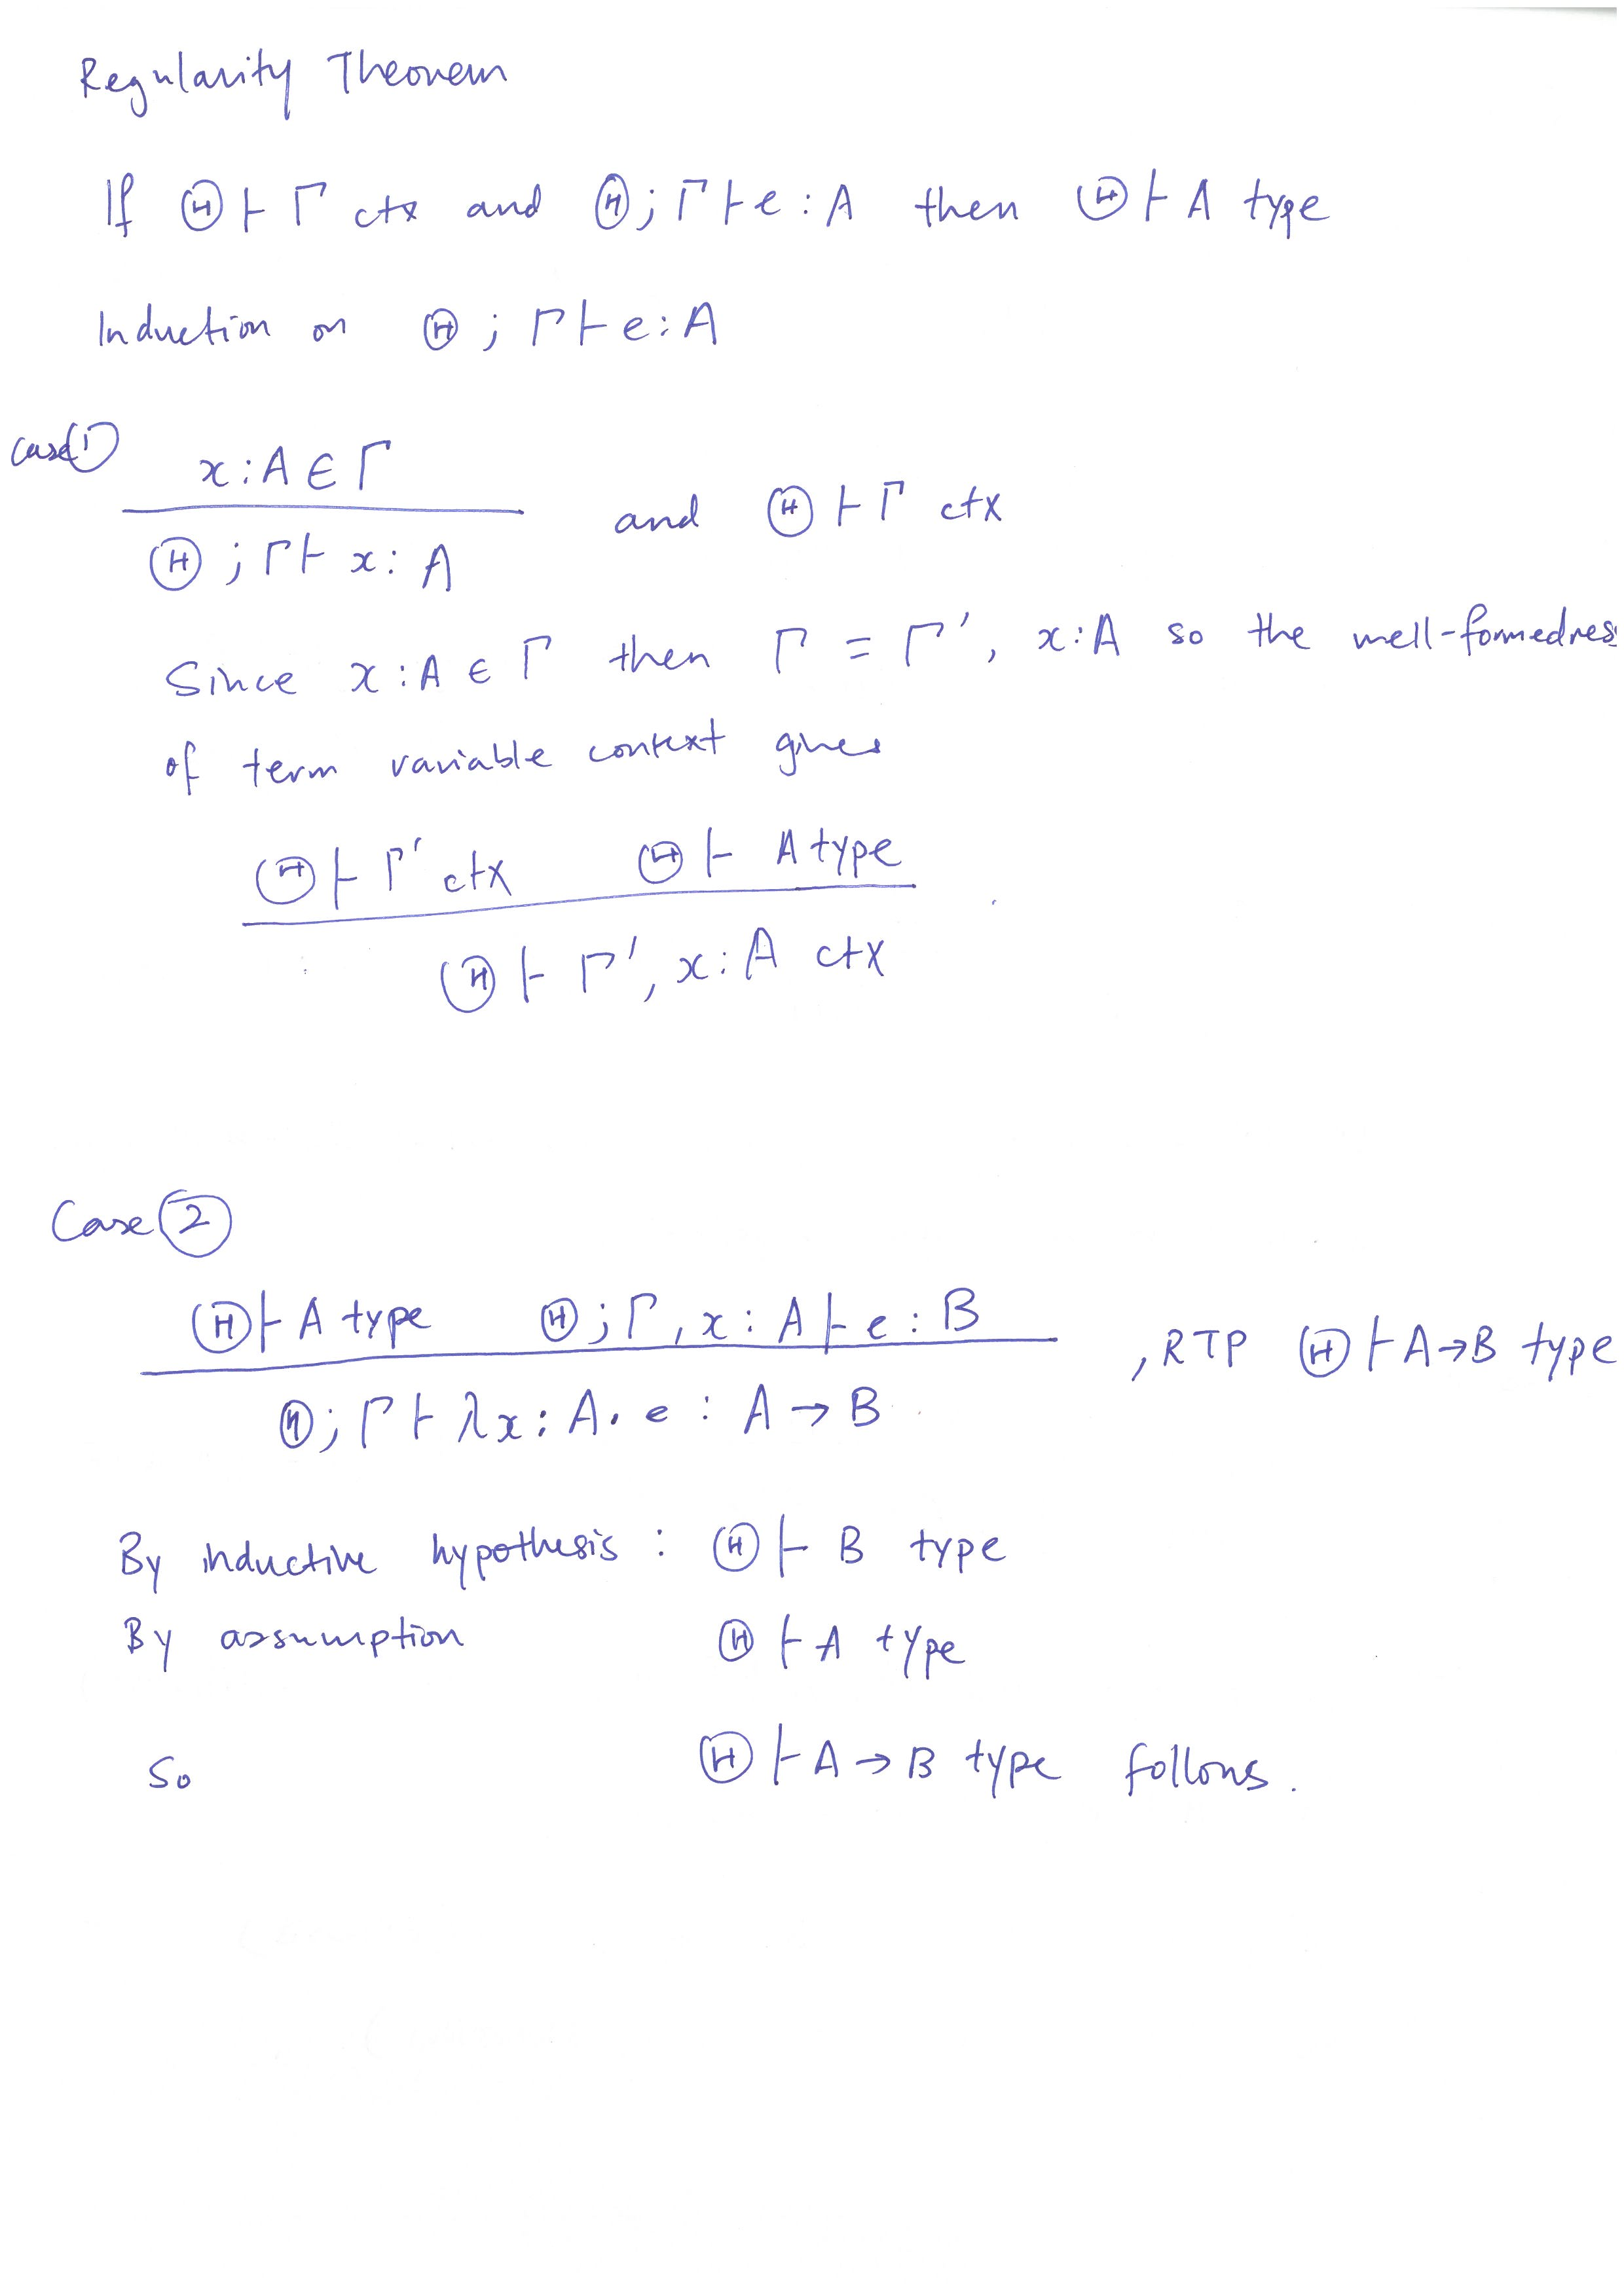
\includegraphics[width=\textwidth]{regularity1.jpg} \\
	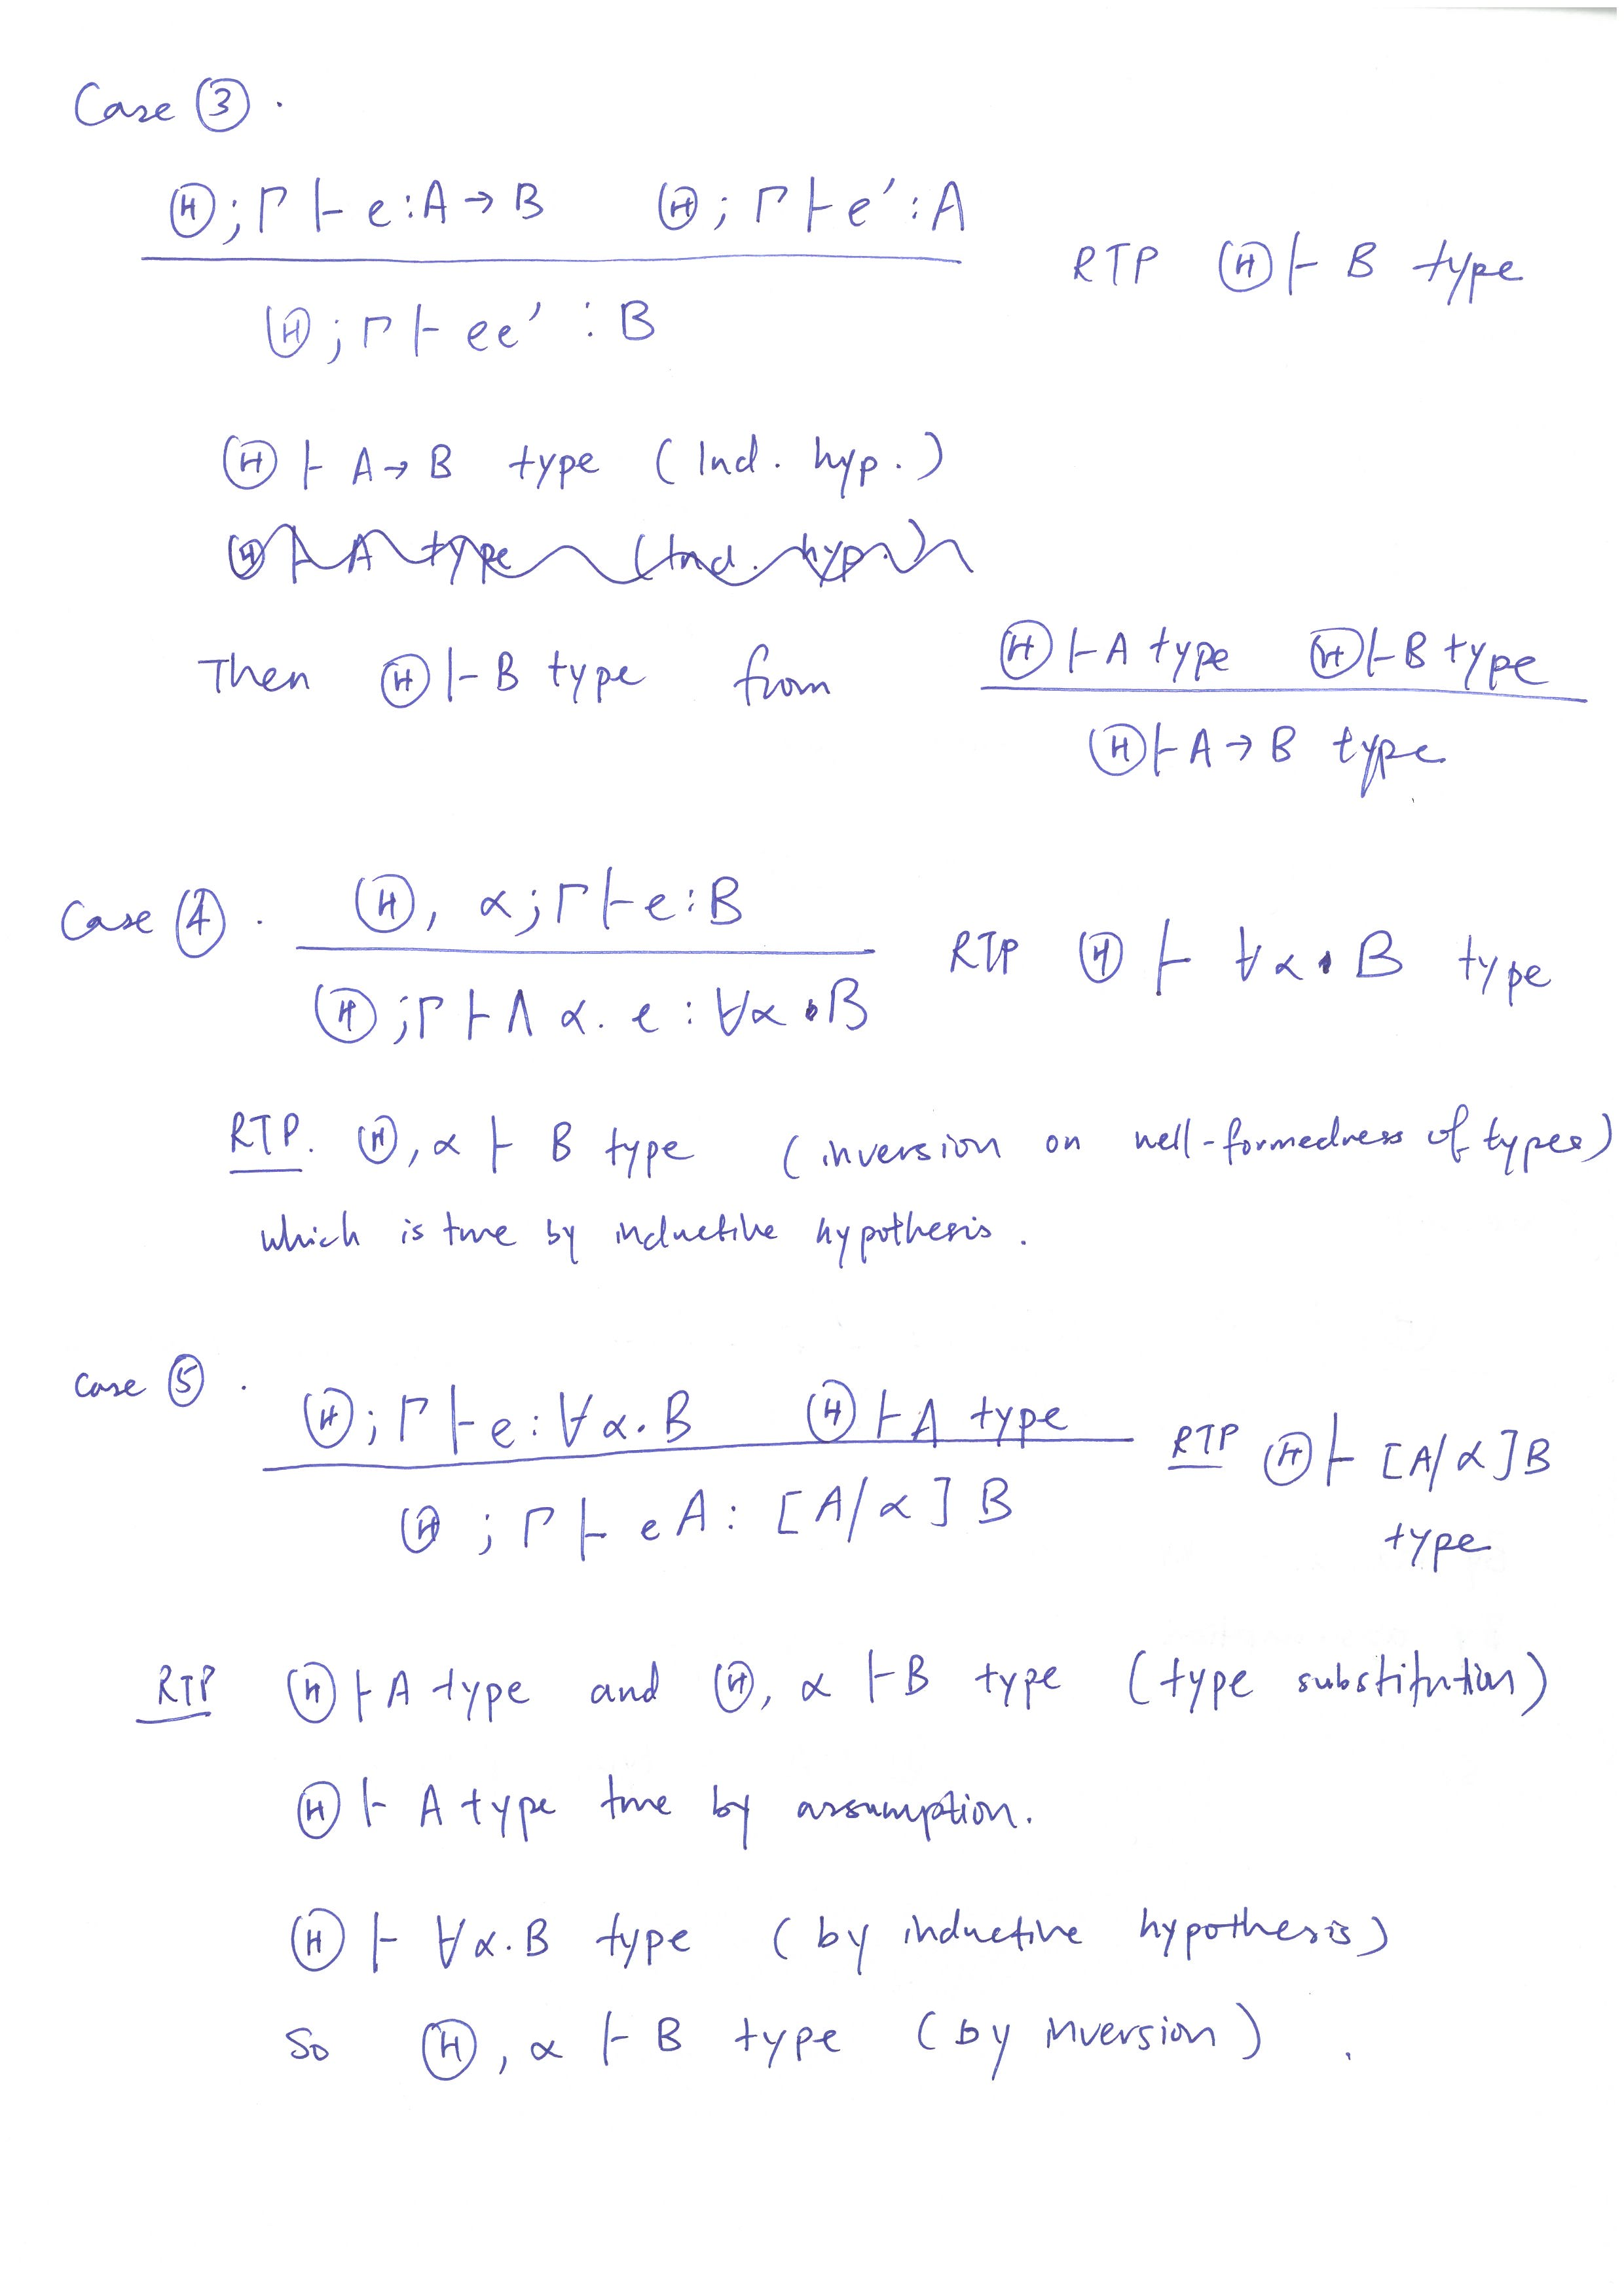
\includegraphics[width=\textwidth]{regularity2.jpg}
	\item Church encoding for unit type: The identity function's type $\forall \alpha. (\alpha \to \alpha)$
	
	\item Church encoding for empty type: $\forall \alpha. \alpha$
	
	\item Church encoding for binary trees: $\forall \alpha.\, \alpha \to (X \to \alpha \to \alpha \to \alpha) \to \alpha$
	
	
\end{enumerate}


\end{enumerate}


\item PYP 2019.9.14

\begin{enumerate}[]
	\item
	 \[
	 \begin{aligned}
	 	\text{Boolean: } & \forall \alpha. \, \alpha \to \alpha \to \alpha \\
	 	\text{True: } &\Lambda \alpha. \, \lambda x : \alpha. \, \lambda y : \alpha. \, x \\
	 	\text{False: } &\Lambda \alpha. \, \lambda x : \alpha. \, \lambda y : \alpha. \, y
	 \end{aligned}
	 \]
	 
	 

\end{enumerate}
\end{enumerate}

\end{document}

